\section{Formation des jets}\label{chapter-JERC-section-jets}
Lorsqu'un parton, \ie\ un quark ou un gluon, est issue de la collision, cette particule possède une haute énergie et $g_s \ll 1$.
Elle radie, par interaction forte, d'autres partons.
Par conservation, l'énergie portée par chaque parton ainsi obtenu diminue et par conséquent, $g_s$ augmente.
\par Tant que l'échelle d'énergie est suffisamment grande pour que $g_s \ll 1$, ce qui correspond à des énergies supérieures à la centaine de \SI{}{\MeV}, il est possible de réaliser des calculs perturbatifs.
La radiation de partons créé la \og gerbe partonique \fg, sujet de la prochaine section.
\par Au fur et à mesure des radiations, l'échelle en énergie diminue et en deçà d'une centaine de \SI{}{\MeV}, il n'est plus possible de réaliser des calculs perturbatifs car $g_s$ augmente.
Des modèles paramétriques sont alors utilisés pour caractériser le phénomène de \og hadronisation \fg, abordés ensuite.

\subsection{Gerbe partonique}\label{chapter-JERC-section-jets-subsec-gerbe-partonique}
%\fullcite{Unorthodox_Introduction_QCD}
Lorsqu'un parton est issu d'une collision au LHC, il se trouve dans un premier temps dans le régime de liberté asymptotique. Il radie alors d'autres partons. Ainsi, pour un événement $\Zboson\to\quark\antiquark$ comme celui de la figure~\ref{subfig-fgraph-Z_q_q} avec deux quarks dans l'état final, il est possible d'obtenir par radiation d'un gluon un état $\quark\antiquark\gluon$ comme ceux illustrés sur les figures~\ref{subfig-fgraph-Z_qg_q} et~\ref{subfig-fgraph-Z_q_qg}, par exemple.
\begin{figure}[h]
\centering\vspace{\baselineskip}
\subcaptionbox{\label{subfig-fgraph-Z_q_q}}[.3\textwidth]
{\begin{fmffile}{Z_q_q}\fmfstraight
\begin{fmfchar*}(30,20)
  \fmfleft{i}
  \fmfright{o1,o3}
  \fmf{boson, tension=2}{i,v1}
  \fmf{phantom}{o1,v1,o3}
  \fmffreeze
  \fmf{fermion}{o1,v1,o3}
  \fmflabel{\Zboson}{i}
  \fmflabel{\quark}{o3}
  \fmflabel{\antiquark}{o1}
  \fmfdot{v1}
\end{fmfchar*}
\end{fmffile}
\vspace{\baselineskip}}
\hfill
\subcaptionbox{\label{subfig-fgraph-Z_qg_q}}[.3\textwidth]
{\begin{fmffile}{Z_qq_q}\fmfstraight
\begin{fmfchar*}(30,20)
  \fmfleft{i}
  \fmfright{o1,o2,o0,o3}
  \fmf{boson, tension=2}{i,v1}
  \fmf{phantom}{o1,v1,o3}
  \fmffreeze
  \fmf{fermion}{o1,v2,v1,o3}
  \fmffreeze
  \fmf{gluon}{v2,o2}
  \fmflabel{\gluon}{o2}
  \fmflabel{\Zboson}{i}
  \fmflabel{\quark}{o3}
  \fmflabel{\antiquark}{o1}
  \fmfdot{v1,v2}
\end{fmfchar*}
\end{fmffile}
\vspace{\baselineskip}}
\hfill
\subcaptionbox{\label{subfig-fgraph-Z_q_qg}}[.3\textwidth]
{\input{\PhDthesisdir/tex/Feynman_diagrams/gerbe_partonique/fgraph-Z_q_qg.tex}\vspace{\baselineskip}}
\caption[Un boson \Zboson\ se désintègre en paire quark-antiquark.]{Un boson \Zboson\ se désintègre en paire quark-antiquark. Dans les cas des figures~\ref{subfig-fgraph-Z_qg_q} et~\ref{subfig-fgraph-Z_q_qg}, un gluon supplémentaire est radié.}
\label{fig-fgraph-Z_q_q_xg}
\end{figure}
\par Il est légitime de se demander quelle est la probabilité d'obtenir un état $\quark\antiquark\gluon$ à partir d'un état $\quark\antiquark$.
Des calculs de section efficace permettent d'obtenir~\cite{salam2010elements}, pour un état initialement à $X$ partons dont un parton $i$ radie un parton $j$,
\begin{equation}
\dd{\sigma_{X+j}} \simeq \sigma_{X} \sum_{i\in\set{X}} \frac{g_s}{2\pi} \frac{\dd{\theta^2}}{\theta^2} \dd{z} P_{ij}(z)
\end{equation}
où $\theta$ est l'angle entre le parton radié $j$ et le parton radiant $i$. La grandeur $P_{ij}(z)$ est la probabilité qu'un parton de type $i$ radie un parton de type $j$ emportant une fraction $z$ de l'énergie initiale de $i$, qui s'exprime
\begin{align}
P_{\quark\quark}(z) &= C_F \frac{1+z^2}{1-z} \msep&
P_{\quark\gluon}(z) &= C_F \frac{1+(1-z)^2}{z} \mend[,]
\\
P_{\gluon\gluon}(z) &= C_A \frac{z^4 + 1 + (1-z)^4}{z(1-z)} \msep&
P_{\gluon\quark}(z) &= T_R (z^2+(1-z)^2) \mend[,]
\end{align}
et $P_{\gluon\antiquark}(z) = P_{\gluon\quark}(z)$,
avec
$C_F=\frac{4}{3}$,
$C_A = 3$ et
$T_R=\frac{1}{2}$.
La probabilité de radier un parton supplémentaire diverge dans deux cas:
\begin{itemize}
\item le parton radié a une énergie faible devant celle du parton radiant, c'est la limite infrarouge;
\item l'angle entre le parton radié et le parton radiant est petit, c'est la limite colinéaire.
\end{itemize}
% Hugues: ces radiations augmentent fortement le nombre de quarks et de gluons dans l’événement et nous le verrons par la suite (partie 3.3.1) nécessite un traitement particulier pour garantir une desciption expérimentale cohé- rente avec l’événement dur.
\par Les nouveaux partons ainsi radiés et les partons initiaux continuent chacun ce processus jusqu'à ce que le phénomène de confinement de couleur réapparaisse. Nous obtenons alors, pour un unique parton directement issu de la collision, une gerbe partonique, \ie\ un ensemble collimé de partons, comme illustré sur la figure~\ref{fig-parton_shower}.
Ce sont ces particules qui vont participer au phénomène de hadronisation dû au confinement de couleur.
\begin{figure}[h]
\centering
\subcaptionbox{Deux quarks sont initialement produits, ce qui correspond au diagramme de la figure~\ref{subfig-fgraph-Z_q_q}.\label{subfig-parton_shower-qq}}[.3\textwidth]
{\begin{tikzpicture}
\def\Lenght{2.5}
\def\qangle{45}
\def\antiqangle{\qangle+180}

\clip (-\Lenght,-\Lenght) rectangle (\Lenght,\Lenght) ;

\fill (0,0) circle (2pt);
\draw (0,0) node [left] {PV} ;

\draw (0,0) --+ (\qangle:\Lenght) node [left] {\quark} ;
\draw (0,0) --+ (\antiqangle:\Lenght) node [right] {\antiquark} ;


\end{tikzpicture}}
\hfill
\subcaptionbox{Un des quarks peut radier un gluon, ce qui correspond au diagramme de la figure~\ref{subfig-fgraph-Z_q_qg}.\label{subfig-parton_shower-qqg}}[.3\textwidth]
{\begin{tikzpicture}
\def\Lenght{2.5}
\def\qangle{45}
\def\antiqangle{\qangle+180}

\clip (-\Lenght,-\Lenght) rectangle (\Lenght,\Lenght) ;

\fill (0,0) circle (2pt);
\draw (0,0) node [left] {PV} ;

\draw (0,0) --+ (\qangle:\Lenght) node [left] {\quark} ;
\draw (0,0) --+ (\antiqangle:\Lenght) node [right] {\antiquark} ;


\def\Lfrac{3}
\draw (0,0) --+ (\qangle:\Lenght/\Lfrac) coordinate (g1) ;
\draw (g1) + (\qangle-30:\Lenght-\Lenght/\Lfrac) coordinate (g2) ;
\draw [decoration={aspect=0.6, segment length=1.75mm, amplitude=1mm,coil},decorate] (g2) -- (g1) ;

\end{tikzpicture}}
\hfill
\subcaptionbox{Le processus est réitéré, donnant un ensemble de particules colorées.\label{subfig-parton_shower-qqNg}}[.3\textwidth]
{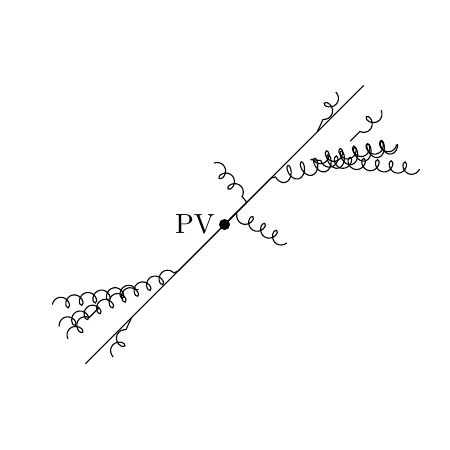
\begin{tikzpicture}
\def\Lenght{2.5}
\def\qangle{45}
\def\antiqangle{\qangle+180}

\clip (-\Lenght,-\Lenght) rectangle (\Lenght,\Lenght) ;

\fill (0,0) circle (2pt);
\draw (0,0) node [left] {PV} ;

\draw (0,0) --+ (\qangle:\Lenght) node [left] {\quark} ;
\draw (0,0) --+ (\antiqangle:\Lenght) node [right] {\antiquark} ;


\def\Lfrac{3}
\draw (0,0) --+ (\qangle:\Lenght/\Lfrac) coordinate (g1) ;
\draw (g1) + (\qangle-30:\Lenght-\Lenght/\Lfrac) coordinate (g2) ;
\draw [decoration={aspect=0.6, segment length=1.75mm, amplitude=1mm,coil},decorate] (g2) -- (g1) ;

\draw (g1) + (\qangle-20:{(\Lenght-\Lenght/\Lfrac)/(\Lfrac/2)}) coordinate (g3) ;
\draw (g3) + (\qangle:{\Lenght-\Lenght/\Lfrac-(\Lenght-\Lenght/\Lfrac)/(\Lfrac/2)}) coordinate (g4) ;
\draw [decoration={aspect=0.8, segment length=1.75mm, amplitude=.75mm,coil},decorate] (g4) -- (g3) ;

\draw (g1) + (\qangle-20:{(\Lenght-\Lenght/\Lfrac)/(\Lfrac)}) coordinate (g3) ;
\draw (g3) + (\qangle-35:{\Lenght-\Lenght/\Lfrac-(\Lenght-\Lenght/\Lfrac)/(\Lfrac)}) coordinate (g4) ;
\draw [decoration={aspect=0.8, segment length=1.75mm, amplitude=.75mm,coil},decorate] (g4) -- (g3) ;

\draw (g3) + (\qangle-50:{\Lenght-\Lenght/\Lfrac-(\Lenght-\Lenght/\Lfrac)/(\Lfrac*2)}) coordinate (g4) ;
\draw [decoration={aspect=0.8, segment length=1.75mm, amplitude=.75mm,coil},decorate] (g4) -- (g3) ;

\draw (g1) + (\qangle:{(\Lenght-\Lenght/\Lfrac)/(2*\Lfrac/3)}) coordinate (g3) ;
\draw (g3) + (\qangle+20:{\Lenght-\Lenght/\Lfrac-(\Lenght-\Lenght/\Lfrac)/(\Lfrac/2)}) coordinate (g4) ;
\draw [decoration={aspect=0.8, segment length=1.75mm, amplitude=.75mm,coil},decorate] (g4) -- (g3) ;

%% qbar shower
\draw (0,0) --+ (\antiqangle:\Lenght/\Lfrac) coordinate (g1) ;
\draw (g1) + (\antiqangle-20:\Lenght-\Lenght/\Lfrac) coordinate (g2) ;
\draw [decoration={aspect=0.8, segment length=1.75mm, amplitude=.75mm,coil},decorate] (g2) -- (g1) ;

\draw (g1) + (\antiqangle-20:{(\Lenght-\Lenght/\Lfrac)/(\Lfrac/2)}) coordinate (g3) ;
\draw (g3) + (\antiqangle:{\Lenght-\Lenght/\Lfrac-(\Lenght-\Lenght/\Lfrac)/(\Lfrac/2)}) coordinate (g4) ;
\draw [decoration={aspect=0.8, segment length=1.75mm, amplitude=.75mm,coil},decorate] (g4) -- (g3) ;

\draw (g1) + (\antiqangle-20:{(\Lenght-\Lenght/\Lfrac)/(\Lfrac)}) coordinate (g3) ;
\draw (g3) + (\antiqangle-35:{\Lenght-\Lenght/\Lfrac-(\Lenght-\Lenght/\Lfrac)/(\Lfrac)}) coordinate (g4) ;
\draw [decoration={aspect=0.8, segment length=1.75mm, amplitude=.75mm,coil},decorate] (g4) -- (g3) ;

%\draw (g3) + (\antiqangle-50:{\Lenght-\Lenght/\Lfrac-(\Lenght-\Lenght/\Lfrac)/(\Lfrac*2)}) coordinate (g4) ;
%\draw [decoration={aspect=0.8, segment length=1.75mm, amplitude=.75mm,coil},decorate] (g4) -- (g3) ;

\draw (g1) + (\antiqangle:{(\Lenght-\Lenght/\Lfrac)/(2*\Lfrac/3)}) coordinate (g3) ;
\draw (g3) + (\antiqangle+20:{\Lenght-\Lenght/\Lfrac-(\Lenght-\Lenght/\Lfrac)/(\Lfrac/2)}) coordinate (g4) ;
\draw [decoration={aspect=0.8, segment length=1.75mm, amplitude=.75mm,coil},decorate] (g4) -- (g3) ;

%% soft gluons
\draw (0,0) --+ (\qangle:.2) coordinate (g1) ;
\draw (g1) + (\qangle-75:.75) coordinate (g2) ;
\draw [decoration={aspect=0.8, segment length=1.75mm, amplitude=.75mm,coil},decorate] (g2) -- (g1) ;

\draw (0,0) --+ (\qangle:.4) coordinate (g1) ;
\draw (g1) + (\qangle+85:.65) coordinate (g2) ;
\draw [decoration={aspect=0.8, segment length=1.75mm, amplitude=.75mm,coil},decorate] (g2) -- (g1) ;

\end{tikzpicture}}

\caption[Formation de deux gerbes partoniques.]{Illustration de la formation de deux gerbes partoniques à partir d'une paire de quarks.}
\label{fig-parton_shower}
\end{figure}

\subsection{Hadronisation}\label{chapter-JERC-section-jets-subsec-hadronisation}
Lorsque des partons en radient d'autres, la conservation de l'énergie implique que chaque particule, individuellement, possède une énergie de plus en plus petite.
Dans le chapitre~\ifref{chapter-MS-MSSM}{\ref{chapter-MS-MSSM}}{sur le modèle standard}, nous avons vu que $g_s$ augmente lorsque l'échelle d'énergie diminue et en-deçà de quelques centaines de \SI{}{\MeV}, $g_s$ diverge.
Le phénomène de confinement de couleur réapparaît et la gerbe partonique subit le phénomène de hadronisation.
Un flux collimé de hadrons, particules de charge de couleur nulle composées de partons, est alors obtenu.
Certains de ces hadrons peuvent comporter des quarks de deuxième ou troisième génération. Ils sont alors instables et peuvent être amenés à se désintégrer, auquel cas ce sont leurs produits de désintégration qui sont observés dans le détecteur.
\par Le phénomène de hadronisation ayant lieu lorsque $g_s\gg1$, il n'est pas possible de réaliser des calculs perturbatifs. Afin de décrire ce phénomène, il faut avoir recours à des modèles paramétriques. Nous en décrivons ici deux, le modèle des cordes de Lund~\cite{Andersson_parton_fragmentation} et le modèle d'agglomération hadronique~\cite{Winter_2004}.
\subsubsection{Modèle des cordes de Lund}\label{chapter-JERC-section-jets-subsec-hadronisation-subsubsec-Lund}
Dans le modèle des cordes de Lund~\cite{Andersson_parton_fragmentation}, les quarks sont reliés en paires $\quark\antiquark$ par des \og cordes \fg{} de couleur, de tension $\kappa \simeq \SI{1}{\GeV.\femto\meter^{-1}}$, comme sur la figure~\ref{subfig-Lund2}. Les gluons sont décrits comme des nœuds des cordes de couleur.
\begin{figure}[h]
\centering
\subcaptionbox{Les deux quarks issus de la collision se séparent à grande vitesse.\label{subfig-Lund1}}[.3\textwidth]
{\begin{tikzpicture}
\draw (-.15,0) node (q1) {} ;
\draw (+.15,0) node (q2) {} ;

\draw [black, fill=ltcolorred3] (q1) circle (3pt);
\draw [black, fill=ltcolorcyan3] (q2) circle (3pt);

\draw [very thick, -latex] (q1) --+ (-.75,0);
\draw [very thick, -latex] (q2) --+ (+.75,0);

\draw (q1) node [above] {\quark};
\draw (q2) node [above] {\antiquark};
\end{tikzpicture}}
\hfill
\subcaptionbox{Une \og corde \fg{} de flux de couleur se forme entre les deux quarks.\label{subfig-Lund2}}[.3\textwidth]
{\begin{tikzpicture}
\draw (-.95,0) node (q1) {} ;
\draw (+.95,0) node (q2) {} ;

\foreach \qa/\qb in {
q1/q2%
}{
\foreach \Dangle in {-15,0,15}{
\draw [thick, ltcolormagenta] (\qa) to  [in=180-\Dangle, out=\Dangle] (\qb);
}
}

\draw [black, fill=ltcolorred3] (q1) circle (3pt);
\draw [black, fill=ltcolorcyan3] (q2) circle (3pt);

\draw [very thick, -latex] (q1) --+ (-.75,0);
\draw [very thick, -latex] (q2) --+ (+.75,0);

\draw (q1) node [above] {\quark};
\draw (q2) node [above] {\antiquark};
\end{tikzpicture}}
\hfill
\subcaptionbox{L'énergie potentielle de la corde est suffisamment grande pour former de nouvelles paires de quarks.\label{subfig-Lund3}}[.3\textwidth]
{\begin{tikzpicture}
\draw (-1.05,0) node (q1) {} ;
\draw (+1.05,0) node (q2) {} ;


\draw (-.25,0) node (q3) {} ;
\draw (+.25,0) node (q4) {} ;

\foreach \qa/\qb in {
q1/q3,%
q4/q2%
}{
\foreach \Dangle in {-15,0,15}{
\draw [thick, ltcolormagenta] (\qa) to  [in=180-\Dangle, out=\Dangle] (\qb);
}
}

\draw [black, fill=ltcolorred3] (q1) circle (3pt);
\draw [black, fill=ltcolorcyan3] (q2) circle (3pt);
\draw [black, fill=ltcoloryellow3] (q3) circle (3pt);
\draw [black, fill=ltcolorblue3] (q4) circle (3pt);

\draw [very thick, -latex] (q1) --+ (-.75,0);
\draw [very thick, -latex] (q2) --+ (+.75,0);

\draw (q1) node [above] {\quark};
\draw (q2) node [above] {\antiquark};
\draw (q3) node [above] {$\antiquark'$};
\draw (q4) node [above] {$\quark'$};
\end{tikzpicture}}

\vspace{\baselineskip}

\subcaptionbox{Le processus se répète tant qu'il y a suffisamment d'énergie pour générer une paire de quarks.\label{subfig-Lund4}}[.45\textwidth]
{\begin{tikzpicture}
\draw (-1.95,0) node (q1) {} ;
\draw (+1.95,0) node (q2) {} ;

\draw (-.45,0) node (q3) {} ;
\draw (+.45,0) node (q4) {} ;

\draw (-1.05,0) node (q5) {} ;
\draw (+1.05,0) node (q6) {} ;

\draw (-1.35,0) node (q7) {} ;
\draw (+1.35,0) node (q8) {} ;

\foreach \qa/\qb in {
q1/q7,%
q5/q3,%
q4/q6,%
q8/q2%
}{
\foreach \Dangle in {-15,0,15}{
\draw [thick, ltcolormagenta] (\qa) to  [in=180-\Dangle, out=\Dangle] (\qb);
}
}

\draw [black, fill=ltcolorred3] (q1) circle (3pt);
\draw [black, fill=ltcolorcyan3] (q2) circle (3pt);
\draw [black, fill=ltcoloryellow3] (q3) circle (3pt);
\draw [black, fill=ltcolorblue3] (q4) circle (3pt);
\draw [black, fill=ltcolorgreen3] (q5) circle (3pt);
\draw [black, fill=ltcoloryellow3] (q6) circle (3pt);
\draw [black, fill=ltcolormagenta3] (q7) circle (3pt);
\draw [black, fill=ltcolorblue3] (q8) circle (3pt);

\draw [very thick, -latex] (q1) --+ (-.75,0);
\draw [very thick, -latex] (q2) --+ (+.75,0);

\draw (q1) node [above] {\quark};
\draw (q2) node [above] {\antiquark};
\draw (q3) node [above] {$\antiquark'$};
\draw (q4) node [above] {$\quark'$};
\draw (q5) node [above] {$\quark''$};
\draw (q6) node [above] {$\antiquark'''$};
\draw (q7) node [above] {$\antiquark''$};
\draw (q8) node [above] {\ $\quark'''$};
\end{tikzpicture}}
\hfill
\subcaptionbox{Des hadrons non colorés sont formés se forment à partir des quarks de basse énergie.\label{subfig-Lund5}}[.45\textwidth]
{\begin{tikzpicture}
\foreach \x/\y in {
1/0,1.1/-.05,%
1.9/.1,2/.15,%
1.4/.2,1.4/.4,1.55/.3,%
-1/0,-1.1/-.05,%
-1.85/.1,-2/.15,-1.95/.035,%
-1.4/.2,-1.25/.3,-1.4/.4%
}
{
\draw [black, fill=ltcolorgray2] (\x,\y-.125) circle (3pt);
}

\draw [very thick, -latex] (-2.25,0) --+ (-.75,0);
\draw [very thick, -latex] (-2.2,-.3) --+ (-.75,-.1);
\draw [very thick, -latex] (-2.25,.3) --+ (-.75,.1);

\draw [very thick, -latex] (2.25,0) --+ (+.75,0);
\draw [very thick, -latex] (2.25,-.3) --+ (+.75,-.1);
\draw [very thick, -latex] (2.25,.3) --+ (+.75,.1);
\end{tikzpicture}}

\caption[Formation de jets dans le cadre du modèle des cordes de Lund.]{Processus de formation de deux jets dans le cadre du modèle des cordes de Lund.}
\label{fig-Lund}
\end{figure}
\par Lorsque deux charges colorées s'éloignent, l'énergie potentielle augmente.
Une fois que l'énergie potentielle est suffisamment grande, une nouvelle paire $\quark'\antiquark'$ est créée (fig.~\ref{subfig-Lund3}), avec une probabilité proportionnelle à $\exp(-\frac{\pi}{\kappa} m_{\quark'})$; la probabilité d'obtenir des quarks lourds par ce processus est donc très faible.
Le partage de l'énergie entre les paires de quarks est régie par une fonction de partition dont les paramètres sont estimés expérimentalement.

\subsubsection{Modèle d'agglomération hadronique}\label{chapter-JERC-section-jets-subsec-hadronisation-subsubsec-agglo_hadronique}
\begin{wrapfigure}{R}{8cm}
\centering
\begin{fmffile}{QCD_clustering_fragmentation}
\begin{fmfchar*}(50,60)
  \fmfleft{i1}
  \fmfrightn{o}{30}
  \fmf{boson,tension=10}{i1,v1}
  \fmf{phantom}{o3,v1,o27}
  \fmffreeze
  \fmf{phantom}{o3,v2}
  \fmf{plain}{v2,v4,v5,v1,v6,v7,v8}
  \fmf{phantom}{v8,o27}
  \fmffreeze
  \fmf{plain}{o1,v2}
  \fmf{plain}{v2,v3,v4,v5,v1,v6,v7,v8}
  \fmf{plain}{v8,o30}
  \fmffreeze
  \fmf{plain}{o3,v9,o4}
  \fmf{plain}{o5,v10,o6}
  \fmf{plain}{v9,v11,v10}
  \fmf{plain}{v11,v12}
  \fmf{plain}{v2,v16,v12,v13}
  \fmf{plain}{v13,v14,v15}
  \fmf{gluon}{v14,v4}
  \fmf{plain}{v15,v17,v17b,o9}
  \fmf{plain}{o10,v17b,o8}
  \fmf{plain,tension=4}{v17,v17c,v18}
  \fmf{plain}{v18,o11}
  \fmf{gluon}{v19,v5}
  \fmf{plain}{v20,v19,v18}
  \fmf{plain}{o16,v20}
  \fmf{plain,tension=4}{v20,v21,v22}
  \fmf{plain}{v22,o18}
  \fmf{plain}{v22,v23}
  \fmf{gluon, tension=2}{v6,v24}
  \fmf{gluon}{v24,v23}
  \fmf{gluon}{v25,v24}
  \fmf{plain}{v23,v26,v27,v28,v25}
  \fmf{plain}{v28,o20}
  \fmf{plain}{v26,v29,o21}
  \fmf{plain}{v29,o22}
  \fmf{plain}{v29,v30,o23}
  \fmf{plain}{v30,o24}
  \fmf{plain}{v25,v31}
  \fmf{plain,tension=4}{v31,v32,v8}
  \fmf{plain}{v31,v33}
  \fmf{plain}{o28,v33,o26}
  \fmfblob{.1w}{v16}
  \fmfblob{.1w}{v17c}
  \fmfblob{.1w}{v21}
  \fmfblob{.1w}{v27}
  \fmfblob{.1w}{v32}
  \fmfdot{v1,v4,v5,v6,v14,v19,v23,v24,v25}
  \fmflabel{ }{o1}
\end{fmfchar*}
\end{fmffile}
\caption[Formation de jets dans le cadre du modèle d'agglomération hadronique.]{Schématisation de l'hadronisation dans le cadre du modèle d'agglomération hadronique.}
\label{fig-agglo_hadronique}
\end{wrapfigure}
Le modèle d'agglomération hadronique~\cite{Winter_2004} repose sur l'hypothèse de conservation des nombres quantiques ainsi que de l'énergie-impulsion entre les partons issus de la gerbe hadronique et les hadrons obtenus après hadronisation.
\par Dans un premier temps, les gluons de la gerbe partonique se désintègrent en paires $\quark\antiquark$. Les partons, uniquement des quarks à ce stade donc, se rassemblent dans un second temps en agglomérats de charge de couleur nulle, c'est le \og pré-confinement \fg.
Deux cas de figurent se présentent alors:
\begin{itemize}
\item la masse de l'agrégat est proche de celle d'un hadron, l'agrégat produit ce hadron;
\item la masse de l'agrégat n'est pas proche de celle d'un hadron et son énergie est supérieure à un seuil $Q_0$, cet agrégat se désintègre en agrégats plus petits et forme plusieurs hadrons.
\end{itemize}
Ce processus est illustré sur la figure~\ref{fig-agglo_hadronique}.
